\section{Action of $\gg$}
\label{sec:Actiongg}
We now turn back to \emph{homology} of $\cms$. In the first subsection we describe geometrically some
homology classes, in order to give some intuition for the following subsections.
In the second subsection we prove Theorem
\ref{thm:Hbms*as*ggrep} in bigradings $(*,m)$ with $*=m$.
In the third subsection we extend the proof to all other bigradings.

\subsection{Geometric examples of homology classes}
In this subsection we consider the surface $\Sigma_{2,1}$, which we abbreviate with $\S$, and
construct some homology classes in $H_2(C_2(\S))$: our aim is to get a first understanding
of why this homology group is isomorphic to $\Sym_2(\H)=\H^{\otimes 2}/\mathfrak{S}_2$.


\subsection{Bigradings of the form $(m,m)$}
In this subsection we construct a $\gg$-~equivariant isomorphism 
\[
\psi_m\colon \Sym_m(\H))\to H_m(\cms).
\]

We already know that these $\Z_2$-vector spaces have the same dimension:
indeed $\Sym_m(\H)$ is precisely the summand in bigrading $(m,m)$ in equation
\eqref{eq:isovectorspaces}, using that a monomial
 whose
weight is \emph{equal} and not bigger than its degree cannot contain factors of the form
$Q^i\epsilon$.

The construction of $\psi_m$ is rather long and technical and involves a few definitions.

\begin{defn}
\label{defn:DinTS} 
Recall Definition \ref{defn:TS}. We denote by $\D\subset\T(\S)\cong\mrS$ the open square $]1/4;3/4[\times]1/2,1[$.
Note that $\D$ is an open disc in $\mrS$ near $\partial\S$ and 
it is disjoint from all $\overline{\U}_i$'s and $\overline{\V}_i$'s. The interior of the surface $\S'$
is then identified with $\T(\S)\setminus [1/4,3/4]\times[1/2,1[$.
\end{defn}


\begin{defn}
\label{defn:cCm}
Let $\cC^m$ be the the (discrete) set of isotopy classes of $m$-tuples of simple closed curves $c_1,\dots,c_m\subset\mrS$
such that any two curves $c_i,c_j$ intersect each other only inside $\D$.
 
Curves are seen as maps $\Sone\to\mrS$, and the intersection of two curves is the intersection of their
images. Here and in the following $\Sone$ is the unit circle in $\C$.

Two $m$-tuples of curves are isotopic if there is an ambient isotopy of $\S$ relative to $\partial\S\cup\D$
transforming one $m$-tuple into the other. In particular $\cC^m$ is more than countable.

An element of $\cC^m$ is called \emph{multicurve}; by abuse of notation the $m$-tuple
$(c_1,\dots,c_m)$ will often represent its class in $\cC^m$, i.e. the corresponding multicurve.
See picture \ref{fig:defcCm}

We denote by $\ZcC{m}$ the free $\Z_2$-vector space with basis $\cC^m$.
There is a canonical surjective map $\pr_m\colon\ZcC{m}\to\Sym_m(\H)$ given by
\[
 \pr_m(c_1,\dots,c_m)=[c_1]\cdot\ldots\cdot[c_m],
\]
where $[c_i]\in\H$ is the fundamental class of the curve $c_i$.

The group $\gg$ acts both on $\ZcC{m}$, by acting on its basis $\cC^m$, and
on $\Sym_m(\H)$, symplectically. The map $\pr_m$ is $\gg$-equivariant.
\end{defn}

\begin{figure}\centering
 \includegraphics[scale=0.7]{defcCm.pdf}
 \caption{A multicurve in $\cC^5$.}
\label{fig:defcCm}
\end{figure}

\begin{defn}
 \label{defn:cmsD}
 Recall Definition \ref{defn:SP}.
 The space $\cmsD$ is the subspace of $\SP^m(\mrS)$ of configurations where all points
 having multiplicity $\geq 2$ lie inside $D$.
 See Figure \ref{fig:defcmsD}.
 
  Note that $\cmsD$ is open in $\SP^m(\mrS)$. There is an open inclusion $\iota_m\colon\cms\subset\cmsD$ and there is a natural map
  \[
  \j_m\colon \ZcC{m}\to H_m(\cmsD)
  \]
  defined as follows: for a class $(c_1,\dots,c_m)\in\cC^m$
  the composition
  \[
   \begin{CD}
    \pa{\Sone}^{\times m} @>c_1\times\dots\times c_m >> (\mrS)^{\times m} @>>> \SP^m(\mrS)
   \end{CD}
  \]
has image in the subspace $\cmsD$; we define $\j_m(c_1,\dots,c_m)$ as the image
of the fundamental class
of the $m$-fold torus in $H_m(\cmsD)$. The result does not change
if we substitute $(c_1,\dots,c_m)$ with another isotopic $m$-tuple of curves in the same multicurve.

We call $[c_1]\cdot\ldots\cdot[c_m]$ the image in the singular chain complex of $\cmsD$ of
the fundamental cycle of the
$m$-fold torus: this cycle represents the class $\j_m(c_1,\dots,c_m)$ and it is \emph{supported}
on the union $c_1\cup\dots\cup c_m$, meaning that it hits configurations in $\cmsD$ of points of $\mrS$
lying in this union.

The group $\Diff(\S,\D\cup\partial\S)$ acts on $\cmsD$, and there is an induced action of $\gg$
on $H_m(\cmsD)$. The map $\j_m$ is $\gg$-equivariant.
\end{defn}

\begin{lem}
 \label{lem:cms->cmsDinj}
 The inclusion $\iota_m\colon\cms\to\cmsD$ induces an injective map
 \[
  \pa{\iota_m}_*\colon H_m(\cms)\to H_m(\cmsD).
 \]
\end{lem}
\begin{proof}
 It is equivalent to prove that the map $\iota_m^*\colon H^m(\cmsD)\to H^m(\cms)$ is surjective,
 or, using Poincaré-Lefschetz duality, that the map $\tH_m(\cmsD^{\infty})\to \tH_m(\cms^{\infty})$
 is surjective: this last map is induced by the map $\cmsD^{\infty}\to\cms^{\infty}$ collapsing the subspace
 $\cmsD^{\infty}\setminus\cms$ to $\infty$.
 
 Recall Lemma \ref{lem:gensymchain} and Definition \ref{defn:gensymchain}. A basis for $\tH_m(\cms^{\infty})$
 is given by classes $[\kappa(0,\uu,\uv)]$, with
 $\uu=(u_1,\dots, u_g)$, $\uv=(v_1,\dots,v_g)$ and
 $\sum_{i=1}^g (u_i+v_i)=m$.
 
 The class $[\kappa(\uu,\uv)]$ is represented by a generalised symmetric chain consisting of only one tuple $\tup=(0,\uu,\uv)$.
 
 In particular there is a map of pairs
 $\phi^{\tup}\colon(\Delta^{\tup},\partial\Delta^{\tup})\to (\cms^{\infty},\infty)$, and the class $[\kappa(\uu,\uv)]$
 is the image along this map of the fundamental class of $H_m\pa{\Delta^{\tup},\partial\Delta^{\tup}}$.
 
 It is straightforward to check that the map $\phi^{\tup}$ factors through
 $(\cmsD,\infty)$, as a map of pairs; surjectivity of $\tH_m(\cmsD^{\infty})\to \tH_m(\cms^{\infty})$ follows.
\end{proof}

We have the following diagram of $\gg$-equivariant maps, where the full arrows are those
that we have already constructed, and we still have to prove the existence of the dashed arrows
\begin{equation}
\label{eq:fulldasheddiagram}
\begin{tikzcd}[column sep=8em,row sep=5em]
  \ZcC{m} \ar[r,"\pr_m",two heads]\ar[d,dashed, swap, "\tpsi_m"]\ar[dr,"\j_m",near start]
  & \Sym_m(\H)\ar[d,dashed ]\ar[dl,dashed,very near start,"\psi_m"]\\
  H_m(\cms)\ar[r,swap,"\pa{\iota_m}*",hook] & H_m\pa{\cmsD}.
 \end{tikzcd}
\end{equation}

We now prove that the map $\j_m$ lifts along $(\iota_m)_*$
to a $\gg$-equivariant map $\tpsi_m$ as in the diagram.
Since $(\iota_m)_*$ is injective by Lemma \ref{lem:cms->cmsDinj}, it suffices to prove that $\j_m$
lands in the image of $(\iota_m)_*$, and this last statement does not depend on how $\gg$ acts on these groups.

We will prove by induction on $m$ the following technical lemma:

\begin{lem}
 \label{lem:tpsiwithproperties}
For each $m$-tuple of curves $(c_1,\dots,c_m)$ representing a class in $\cC^m$
and for each open neighborhood $\N\subset\mrS$ of
$\D\cup c_1\cup\dots\cup c_m$, there is a singular cycle $\fc=\tpsi_m(c_1,\dots,c_m)$
in $\cms$ with the following properties:
\begin{itemize}
 \item the cycle $\fc$ is \emph{supported} on $\N$, i.e.,
this singular cycle only hits configurations of $m$ distinct points of $\mrS$ that actually lie in $\N$;
\item $\pa{\iota_m}_*(\fc)$ represents the homology class $\j_m(c_1,\dots,c_m)\in H_m\pa{\cmsD}$;
\item the two cycles $\pa{\iota_m}_*(\fc)$ and $[c_1]\cdot\ldots\cdot[c_m]$
are connected by a homology in $\cmsD$ which is supported on $\N$ (the word
\emph{homology} denotes here a $(m+1)$-singular chain whose boundary is the difference between the two cycles).
\end{itemize}
\end{lem}

For $m=0$ both $\ZcC{0}$ and $H_0(C_0(\S))$ are
isomorphic to $\Z_2$ and there is nothing to show. For $m=1$
we have a canonical identification $H_1(C_1(\S))\simeq\H\simeq\Sym_1(\H)$, so we take $\tpsi_1=\pr_1$;
obviously for all $c_1$ representing a class in $\cC^1$, the homology class $\pr_1(c_1)\in\H$
is represented by a cycle supported on $c_1$,
and in this case the cycles $\iota_*\pa{\tpsi(c_1)}$ and $\pr_1(c_1)=\j_m(c_1)$ coincide.

Let now $m\geq 1$ and in the following fix a class $(c_1,\dots, c_{m+1})\in\cC^{m+1}$.

\begin{defn}
\label{defn:variationsCm}
We introduce several variations of the notion of configuration space; see Figure \ref{fig:defcmsD}.
\begin{itemize} 
 \item The space $C_{1,m}(\S)$ is the subspace of $\mrS\times \cms$ containing all configurations
 $\pa{\bar P;\set{P_1,\dots,P_m}}$ with $\bar P\neq P_i$ for all $i$; in other words it is
 the space of configurations of $m+1$ points, one of which is \emph{white} (meaning that
 it is distinguishable from the other points), whereas the other are \emph{black} and not distinguishable
 from each other.
 \item The space $\fmstwoD$ is the subspace of $\mrS\times\cms$ containing all configurations
 $\pa{\bar P;\set{P_1,\dots, P_m}}$ where either $\bar P\in\D$ may coincide with \emph{exactly}
 one $P_i$, or
 $\bar P\not\in \D$ must be distinct from all $P_i$'s.
 Again $\bar P$ is called the white point.
 \item The space $\cmstwoD$ is the subspace of $\SP^{m+1}(\mrS)$ of configurations where either all $m+1$ points
 are distinct, or there is exactly one point \emph{inside $\D$} with multiplicity $2$ and $m-1$ other points,
 somewhere in $\mrS$, with multiplicity $1$.
\end{itemize}
 \end{defn}
 
\begin{figure}\centering
 \includegraphics{defcmsD.pdf}
 \caption{A configuration in each of the space introduced in Definitions \ref{defn:cmsD} and \ref{defn:variationsCm}.
 Whenever a multiplicity is not specified, it is equal to 1.}
\label{fig:defcmsD}
\end{figure}

 
We have the following inclusions:
\[
C_{1,m}(\S)\subset\fmstwoD\subset\mrS\times\cmsD\subset\mrS\times\SP^m(\mrS);
\]
\[
C_{m+1}(\S)\subset\cmstwoD\subset C_{m+1}^{\D}(\S)\subset\SP^{m+1}(\mrS).
\]
All these spaces are
manifolds of dimension $2m+2$ and all inclusions are open.

In particular there is a sequence of maps
\[
 H_{m+1}\pa{C_{m+1}(\S)}\to H_{m+1}\pa{\cmstwoD}\to H_{m+1}\pa{C_{m+1}^{\D}(\S)}
\]
and we will first lift the homology class $j_{m+1}(c_1,\dots,c_{m+1})$ to $H_m\pa{\cmstwoD}$ and
then to $H_{m+1}(C_{m+1}(\S))$, each time controlling the support of our representing
cycles and of the homologies between them.

Fix a neighborhood $\N$ of $\D\cup c_1\cup\dots\cup c_{m+1}$.

For the first lift, let $\N'=\pa{\N\setminus c_1}\cup\D$, which is an open
neighborhood of $\D\cup c_2\cup\dots\cup c_{m+1}$ in $\mrS$. By inductive hypothesis
there is a cycle $\fc=\tpsi_m(c_2,\dots,c_{m+1})$ in $\cms$ which is supported on $\N'$,
and such that $(\iota_m)_*(\fc)$ is homologous to $[c_2]\cdot\ldots\cdot[c_{m+1}]$
along a homology in $\cmsD$ supported on $\N'$ as well.

We can multiply both
cycles and the homology between them by the cycle $[c_1]$: the result are the two homologous cycles
$[c_1]\cdot \fc$ and $[c_1]\cdot\ldots\cdot[c_{m+1}]$ in $C_{m+1}^{\D}(\S)$: both cycles and the
homology between them are supported on $\N$. Note now that the
cycle $[c_1]\cdot\fc$ lives in $\cmstwoD$, so the first lift is done and we can now
deal with the second lift.

There is a natural map $\p\colon \fmstwoD\to \cmstwoD$, which converts the white point
into a black point. This map restricts to %maps $\fmstwoD\to\cmstwoD$ and 
a map $C_{1,m}(\S)\to C_{m+1}(\S)$, so that
we have a commutative diagram
 \begin{equation}\label{eq:cmstwodiagram}
  \begin{CD}
   C_{1,m}(\S) @>\subset >> \fmstwoD
\\   @V\p VV @V\p VV
\\   C_{m+1}(\S) @>\subset >> \cmstwoD
   \end{CD}
\end{equation}

\begin{defn}
\label{defn:falsediagonals} 
Let 
\[
\Dmone=\cmstwoD\setminus C_{m+1}(\S)
\]
and similarly
\[
\Donem=\fmstwoD\setminus C_{1,m}(\S).
\]
We note that $\p$ restricts to a homeomorphism $\Donem\to\Dmone$. Moreover both $\Dmone\subset\cmstwoD$
and $\Donem\subset\fmstwoD$ are closed submanifolds of codimension $2$, and the map $\p$ restricts to
a $2$-fold ramified covering between their respective normal bundles.
\end{defn}

Diagram \eqref{eq:cmstwodiagram} induces a commutative diagram in homology
\begin{equation}
 \label{eq:fivediagram}
\minCDarrowwidth15pt
 \begin{CD}
  @. H_{m+1}\pa{\fmstwoD} @>>> H_{m+1}\pa{\fmstwoD, C_{1,m}(\S)}\\
  @. @V\p_*VV @V\p_*VV\\
  H_{m+1}\pa{ C_{m+1}(\S)} @>>> H_{m+1}\pa{\cmstwoD} @>>> H_{m+1}\pa{\cmstwoD,C_{m+1}(\S)}
 \end{CD}
\end{equation}

Recall that we want lift the homology class represented by the cycle $[c_1]\cdot\fc$
from the bottom central group to the bottom left group.

We first note that there is a lift of $[c_1]\cdot\fc$ to a cycle $[c_1]\otimes\fc$ in $\pa{\fmstwoD}$:
this is defined by declaring the point in $[c_1]\cdot\fc$ that spins around $c_1$
to be white. We then note that the right vertical map
\[
\p_*\colon H_{m+1}\pa{\fmstwoD, C_{1,m}(\S)} \to H_{m+1}\pa{\cmstwoD,C_{m+1}(\S)}
\]
can be rewritten, after using excision to tubular neighborhoods of $\Donem$ and $\Dmone$ respectively,
and the Thom isomorphism, as a map
\[
 H_{m-1}(\Donem)\to H_{m-1}(\Dmone).
\]
The latter map is multiplication by $2$, after identifying $\Dmone$ and $\Donem$ along $p$:
indeed the normal bundle of $\Donem$ is a
double covering of the normal bundle of $\Dmone$, hence the Thom class of the first disc
bundle corresponds to twice the Thom class of the second disc bundle. We are working
with coefficients in $\Z_2$, so multiplication by $2$ is the zero map.

Therefore the image of the cycle $[c_1]\otimes \fc$ along the diagonal of the square
in diagram \eqref{eq:fivediagram} is zero; hence the image of $[c_1]\cdot\fc$ in $H_{m+1}\pa{\cmstwoD,C_{m+1}(\S)}$
is zero; hence the homology class of $[c_1]\cdot\fc$ comes from $H_{m+1}(C_{m+1}(\S))$. More
precisely, there exists a cycle $\fc'$ in $C_{m+1}(\S)$ such that $\pa{\iota_{m+1}}_*(\fc')$ is homologous
to $[c_1]\cdot\fc$.

To prove Lemma \ref{lem:tpsiwithproperties} we need to find a good cycle and
a good homology, namely two that are supported on $\N$: a priori both $\fc'$ and the homology
between $\pa{\iota_{m+1}}_*(\fc')$ and $[c_1]\cdot\fc$ are only supported on $\mrS$.

This can be done by replacing, in the whole argument of the proof, the surface $\mrS$ with the surface $\N$.
We can define configuration spaces as in Definition \ref{defn:variationsCm} also for the open surface
$\N$, and we can repeat the argument considering $\N$ as the \emph{ambient surface}:
indeed we only needed a surface containing $\D$ and all curves $c_1,\dots,c_{m+1}$.

It is crucial that the action of $\gg$ is not involved in the statement of Lemma
\ref{lem:tpsiwithproperties}, as $\N\subset\S$ is not preserved, even up to isotopy,
by diffeomorphisms of $\S$.
Lemma \ref{lem:tpsiwithproperties} is proved.

We now have to prove the following lemma to conclude the proof of Theorem \ref{thm:Hbms*as*ggrep}
in bigradings $(m,m)$.
\begin{lem}
 \label{lem:tpsi->psi}
The map $\tpsi_m\colon\ZcC{m}\to H_m(\cms)$ is surjective and factors through the map $\pr_m$.
\end{lem}
\begin{proof}
The factorisation is equivalent to the inclusion $\ker\pr_m\subseteq\ker\tpsi_m$: since both
$\pr_m$ and $\tpsi_m$
are $\gg$-equivariant, also the induced map of vector spaces
\[
\Sym_m(\H)=\ZcC{m}/\ker\pr_m\to H_m(\cms)
\]
will automatically be
$\gg$-equivariant.

Recall from the proof of Lemma \ref{lem:cms->cmsDinj} that a basis for $\tH_m(\cms^{\infty})$ 
is given by the classes $[\kappa(\uu,\uv)]$, represented by generalised
symmetric chains consisting of only one tuple $\tup=(0,\uu,\uv)$, for some vectors
$\uu=(u_1,\dots,u_g)$ and $\uv=(v_1,\dots,v_g)$ satisfying $\sum_{i=1}^g(u_i+v_i)=m$.

The homology class
$[\kappa(\uu,\uv)]$ is the fundamental class
of the sphere $e^{\tup}\cup\set{\infty}\subset\cms^{\infty}$: the inclusion of this sphere in $\cms^{\infty}$
restricts to a proper embedding $e^{\tup}\subset\cms$.

By Poincaré Lefschetz duality $\tH_m(\cms^{\infty})\simeq H^m(\cms)$, and the latter is
the dual of $H_m(\cms)$.

We can therefore associate to $[\kappa(\uu,\uv)]$ a linear functional
on $H_m(\cms)$. This is the algebraic intersection product with the cell $e^{\tup}$, seen as a proper submanifold of $\cms$:
we denote it by
\[
 \cdot\cap e^{\tup}\colon H_m(\cms)\to\Z_2.
\]
Therefore
\[
 \ker\tpsi_m=\bigcap_{\tup}\ker\pa{(\cdot\cap e^{\tup})\circ\tpsi_m},
\]
and it suffices to check that $\ker\pr_m\subseteq\ker\pa{(\cdot\cap e^{\tup})\circ\tpsi_m}$
for all $\tup$ of the form $(0,\uu,\uv)$, or equivalently, that $(\cdot\cap e^{\tup})\circ\tpsi_m$ factors through $\pr_m$.

Recall from the proof of Lemma \ref{lem:cms->cmsDinj} that the cohomology class $(\cdot\cap e^{\tup})$ on $\cms$ is a pullback
of a cohomology class of $\cmsD$, that we call $(\cdot\cap e^{\tup})^{\D}$. Alternatively,
note that the inclusion $e^{\tup}\cap \set{\infty}\to\cms^{\infty}$ is the composition of the inclusion $e^{\tup}\cap\set{\infty}\to\cmsD^{\infty}$
and the quotient map $\cmsD^{\infty}\to\cms^{\infty}$, and consider the fundamental class of the sphere $e^{\tup}\cup\set{\infty}$ and its images.

We can therefore compute the map $(\cdot\cap e^{\tup})\circ\tpsi_m$ as the map 
\begin{equation}
\label{eq:badformula}
(\cdot\cap e^{\tup})^{\D}\circ\j_m\colon \ZcC{m}\to\Z_2.
\end{equation}
The latter map coincides with the composition
\begin{equation}
 \label{eq:productformula}
\pa{ \prod_{i=1}^g(\cdot\cap\U_i)^{u_i}(\cdot\cap\V_i)^{v_i}}\circ\pr_m,
\end{equation}

where $\prod_{i=1}^g(\cdot\cap\U_i)^{u_i}(\cdot\cap\V_i)^{v_i}\in\Sym_m(\Hom(\H;\Z_2))=\Hom\pa{\Sym_m(\H);\Z_2}$.

This can be checked on every generator $(c_1,\dots, c_m)\in\ZcC{m}$ by chosing in the isotopy class a representative $(c_1,\dots, c_m)$
with all curves $c_i$ transverse to all segments $\U_j$ and $\V_j$.

Consider again the map $c_1\times\dots\times c_m\colon \pa{\Sone}^{\times m}\to\cmsD$ that we used to define the cycle $[c_1]\cdot\dots[c_m]$
representing the class $\j_m(c_1,\dots,c_m)$ (see Definition \ref{defn:cmsD}):
this map is an embedding near $e^{\tup}$ and is transverse to $e^{\tup}$.

The equality of the maps in equations \eqref{eq:badformula} and \eqref{eq:productformula} on the generator $(c_1,\dots,c_m)\in\ZcC{m}$
follows from a straightforward
computation (in $\Z_2$) of the cardinality of the set $[c_1]\cdot\dots[c_m]\cap e^{\tup}$ in terms
of the cardinalities of all sets of the form $c_i\cap\U_j$ and $c_i\cap \V_j$.
In particular $(\cdot\cap e^{\tup})\circ\tpsi_m$ factors through $\pr_m$.

To show surjectivity of $\tpsi_m$, choose a tuple $\tup$ of the form $(0,\uu,\uv)$
and an $m$-tuple of curves $(c_1,\dots,c_m)$ containing, for every $1\leq i\leq g$, $u_i$ parallel
copies of some curve representing $\u_i$ and $v_i$ parallel copies of some curve representing
$\v_i$ (see Definition \ref{defn:dualHbasis}), such that all intersections between these curves
lie in $\D$.

Then $j_m(c_1,\dots,c_m)\cap e^{\tup}=1$ and for all
other tuples $\tup'$ of the form $(0,\uu',\uv)$ we have instead $j_m(c_1,\dots,c_m)\cap e^{\tup'}=0$.

This shows that $\psi_m(c_1,\dots,c_m)=[c_1]\cdot\ldots\cdot[c_m]\in\Sym_m(\H)$, which is
one of the generating monomials.
\end{proof}

Theorem \ref{thm:Hbms*as*ggrep} is now proved in all bigradings of the form $(m,m)$.

\subsection{General bigradings $(m-l,m)$.} Fix $0\leq l\leq m$ for the whole subsection: our next aim is to prove Theorem
\ref{thm:Hbms*as*ggrep} for the bigrading $(m-l,m)$.

For all $0\leq p\leq m$, the group $\Diff(\S;\partial\S\cup\D)$ acts both on $C_p(\D)\times C_{m-p}(\S')$
and on $\cms$, and the map $\mu$ is equivariant with respect to this action
(see Definition \ref{defn:universalSbundle});
hence, using the K\"{u}nneth formula, there is an induced $\gg$-equivariant map in homology
\begin{equation}
 \label{eq:mu*}
 \mu_*\colon H_{p-l}\pa{C_p(\D)}\otimes H_{m-p}\pa{C_{m-p}(\S')}\to H_{m-l}\pa{\cms}.
\end{equation}

Note that $H_{p-l}\pa{C_p(\D)}\otimes H_{m-p}\pa{C_{m-p}(\S')}$
is the tensor product of the trivial representation $H_{p-l}\pa{C_p(\D)}$, and
of the representation $H_{m-p}\pa{C_{m-p}(\S')}$, which by the results of the previous
section is isomorphic to the symplectic representation $\Sym_{m-p}(\H)$.

We will prove the following lemma, from which Theorem \ref{thm:Hbms*as*ggrep} follows:
\begin{lem}
 \label{lem:oplussplitting}
For all $l\leq p\leq m$ the map $\mu_*$ in equation \eqref{eq:mu*} is injective, and the collection
of all these maps yields a splitting
\begin{equation}
  \label{eq:musplitting}
 H_{m-l}(\cms)=\bigoplus_{p=l}^m H_{p-l}\pa{C_p(\D)}\otimes H_{m-p}\pa{C_{m-p}(\S')}.
\end{equation}
\end{lem}
\begin{proof}
Note that the statement of the lemma does not depend on the the action of $\gg$:
we have a map from the right-hand side to the left-hand side of equation \eqref{eq:musplitting},
we already know that it is $\gg$-equivariant,
we only need to show that it is a linear isomorphism. Note also that Lemma \ref{lem:gensymchain}
implies that the two vector spaces have the same dimension.

Fix $l\leq p\leq m$ and $\ualpha=(\alpha_j)_{j\geq 0}$, and let $[a]=Q^{\ualpha}\epsilon=\prod_{j=0}^{\infty}(Q^j\epsilon)^{\alpha_j}$ be a generator of
$H_{p-l}(C_p(\D))$, hence $l=\sum_j\alpha_j$ and $p=\sum_j\alpha_j2^j$.

Fix also $\uu=(u_1,\dots, u_g)$ and $\uv=(v_1,\dots,v_g)$,
and let $[b]=\u^{\uu}\cdot\v^{\uv}=\prod_{i=1}^g (\u_i^{u_i}\v_i^{v_i})$ be a generator of $H_{m-p}(C_{m-p}(\S'))$, using the
isomorphism proved in the previous subsection, with $(m-p)=\sum_i(u_i+v_i)$.

Here $a$ and
$b$ are chosen singular cycles representing the homology classes, with $a$ supported on $\D$
and $b$ supported on $\S'$. See Figure \ref{fig:axb}

\begin{figure}\centering
 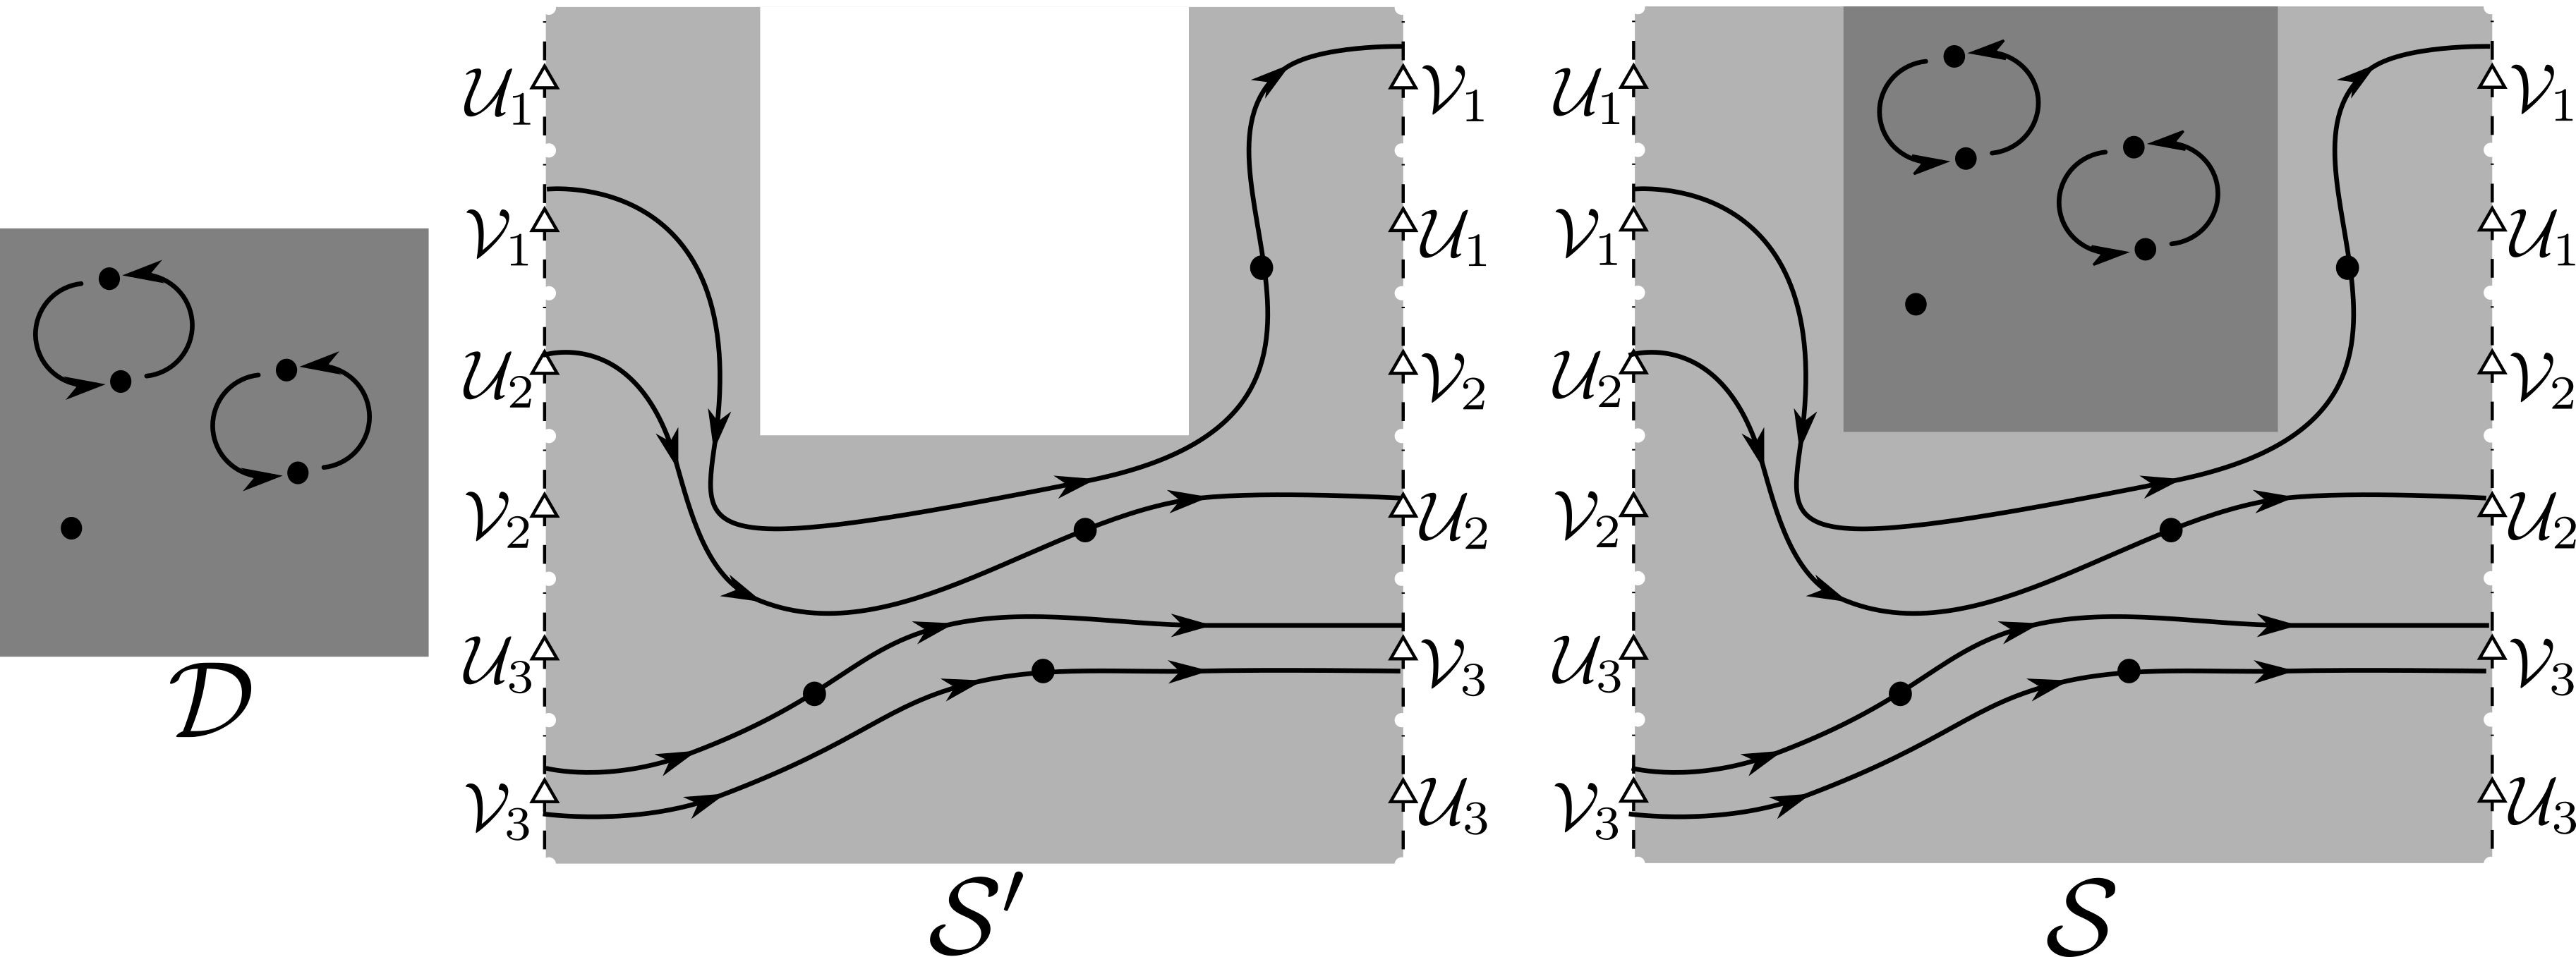
\includegraphics[scale=0.65]{axb.pdf}
 \caption{From left to right, the class $[a]=\epsilon\cdot(Q\epsilon)^2\in H_2(C_5(\D))$;
 the class $[b]=\v_1\cdot\u_2\cdot\v_3^2\in H_4(C_4(\S'))$; and the product class
 $\mu_*([a]\otimes[b])\in H_6(C_9(\S))$.}
\label{fig:axb}
\end{figure}

Then $[a]\otimes [b]$ is a generator of $H_{p-l}(C_p(\D))\otimes H_{m-p}(C_{m-p}(\S'))$,
by the K\"unneth formula, and we are interested in the homology class $\mu_*([a]\otimes [b])$.

There is one such
class for any choice of $[a]$ and $[b]$ as above, that is, for any choice of
$p$, $\ualpha$, $\uu$ and $\uv$ satisfying the conditions
$l=\sum_{j\geq 0}\alpha_j$, $p=\sum_{j\geq 0}\alpha_j2^j$ and $(m-p)=\sum_{i=1}^g(u_i+v_i)$, where
we use the notation above.

We want to show that the collection of all the corresponding classes of the form $\mu_*([a]\otimes [b])$
gives a basis for $H_{m-l}(\cms)$.

We will study
the intersection of $\mu_*([a]\otimes [b])$ with cohomology classes of $\cms$ represented by
generalised symmetric chains in $\cms^{\infty}$.

To compute the algebraic intersection
between $\mu_*([a]\otimes [b])$ and $[\kappa(p',\ualpha',\uu',\uv')]$ we
consider the map
\[
 \mu^{\infty}\colon \cms^{\infty}\to \pa{C_p(\D)\times C_{m-p}(\S')}^{\infty}
\]
which collapses to $\infty$ the complement in $\cms^{\infty}$ of the open submanifold $C_p(\D)\times C_{m-p}(\S')$.

By Poincaré-Lefschetz duality, the map $\mu^{\infty}_*$ in reduced homology corresponds to the cohomology map
\[
 \mu^*\colon H^*(\cms)\to H^*(C_p(\D)\times C_{m-p}(\S'))=H^*(C_p(\D))\otimes H^*(C_{m-p}(\S')).
\]

We give $\pa{C_p(\D)\times C_{m-p}(\S')}^{\infty}$ the cell complex structure of the smash product
$C_p(\D)^{\infty}\wedge C_{m-p}(\S')^{\infty}$. Here $C_p(\D)^{\infty}$ is given the cell structure of $C_p((0,1)^2)^{\infty}$
coming from the natural identification $\D=]1/4,3/4[\times]1/2,1[\cong]0,1[^2$, which is obtained by rescaling
and translating. Moreover we choose any diffeomorphism $\mrS'\cong\mrS$ that restricts to the identity
on all $\U_i$'s and $\V_i$'s, and give $C_{m-p}(\S')^{\infty}$ the cell structure of $C_{m-p}(\S)^{\infty}$.

Recall that $\cms^{\infty}$ can be filtered according to the norm of cells: a cell $e^{\tup}$ associated with
the tuple $\tup=(l,\ux,\uu,\uv)$ has norm $\sum_{i=1}^l x_i$, and the norm is weakly decreasing along boundaries.
In the previous section we just considered
the associated filtration of the reduced chain complex $\tCh_*(\cms^{\infty})$, whereas now we
consider the closed subcomplex $F_p\cms^{\infty}\subset\cms^{\infty}$, which is the union
of all cells of norm $\leq p$.

The crucial observation is that $\mu^{\infty}$ restricts to a cellular map 
\[
F_p\cms^{\infty}\to \pa{C_p(\D)\times C_{m-p}(\S')}^{\infty}.
\]

To see this, fix a tuple $\tilde{\tup}=(\tilde{l}, \tilde{\ux},\tilde{\uu},\tilde{\uv})$ of norm $\tilde{p}\leq p$
and of dimension $\tilde{l}+m$, and
consider the open cell
cell $e^{\tilde{\tup}}\subset F_p\cms^{\infty}$.

If $\tilde{p}<p$, then
$e^{\tilde{\tup}}\cap (C_p(\D)\times C_{m-p}(\S'))$ is empty. If $\tilde{p}=p$, then
\[
e^{\tilde{\tup}}\cap (C_p(\D)\times C_{m-p}(\S'))=e^{\tup'}\times e^{\tup''},
\]
where $\tup'=(\tilde{l},\tilde{\ux})$ and $\tup''=(0,\tilde{\uu},\tilde{\uv})$.

Therefore
$\mu^{\infty}(e^{\tilde{\tup}})$ is $\set{\infty}$ in the first case, and in the second case it
is contained in the union $\set{\infty}\cup e^{\tup'}\times e^{\tup''}$, which is also
contained in the $(\tilde{l}+m)$-skeleton of $\pa{C_p(\D)\times C_{m-p}(\S')}^{\infty}$.

Consider now the generalised symmetric chain $\kappa(p',\ualpha',\uu',\uv')$ representing
a class in $\tH_{m+l}(\cms^{\infty})=H^{m-l}(\cms)$, with $\ualpha'=(\alpha'_j)_{j\geq 0}$,
$\uu'=(u_1,\dots,u'_g)$ and $\uv'=(v'_1,\dots,v'_g)$; in particular $l=\sum_{j\geq 0}\alpha'_j$.
Suppose moreover $p'\leq p$.

If $p'<p$, the previous argument shows that $\mu^{\infty}_*\pa{\kappa(p',\ualpha',\uu',\uv')}=0$
in the reduced cellular chain complex,
and in particular the corresponding homology class is mapped to zero.

Suppose now $p'=p$: then the previous argument shows that
the homology class $[\kappa(p',\ualpha',\uu',\uv')]\in \tH_{m+l}(\cms^{\infty})$
is mapped along $\mu^{\infty}_*$ to the class
\[
[\kappa(\ualpha')]\otimes [\kappa(\uu',\uv')]\in\tH\pa{C_p(\D)^{\infty}\wedge C_{m-p}(\S')^{\infty}}.
\]
Indeed each tuple $\tup$ in the cycle $\kappa(p',\ualpha',\uu',\uv')|$ is mapped by $\mu^{\infty}_*$
to a corresponding pair of tuples $\tup'\otimes\tup''$ in the cycle $\kappa(\ualpha')\otimes \kappa(\uu',\uv')$,
so even at the level of chains we have
\[
\mu^{\infty}_*\pa{\kappa(p',\ualpha',\uu',\uv')}=\kappa(\ualpha')\otimes \kappa(\uu',\uv').
\]

We can now compute the algebraic intersection of $\mu_*([a]\otimes [b])$ with
the cohomology class $[\kappa(p',\ualpha',\uu',\uv')]$ as the algebraic intersection between
$[a]\otimes [b]$ and $\mu^{\infty}_*\pa{[\kappa(p',\ualpha',\uu',\uv')]}$.

For $p'<p$ the previous argument show that this intersection is zero.

For $p'=p$ the intersection between
$[a]\otimes [b]$ and $\mu^{\infty}_*([\kappa(p,\ualpha',\uu',\uv')])=[\kappa(\ualpha')]\otimes [\kappa(\uu',\uv')]$
is $1\in\Z_2$ exactly when $\ualpha=\ualpha'$, $\uu=\uu'$ and $\uv=\uv'$; otherwise it is $0$.

To finish the proof we consider the collection of all strings of the form
\[
\pa{p,\ualpha=(\alpha_j)_{j\geq 0},\uu=(u_1,\dots,u_g),\uv=(v_1,\dots,v_g)}
\]
satisfying $l=\sum_j\alpha_j$,$p=\sum_j \alpha_j2^j$ and $(m-p)=\sum_i(u_i+v_i)$;
we choose a total order on the set of these strings,
such that the parameter $p$ is weakly increasing along this order; we associate
to each string its corresponding class in $H_{m-l}(\cms)$ of the form $\mu_*([a]\otimes [b])$ and its
corresponding class $[\kappa(p,\ualpha',\uu',\uv')]\in\tH_{m+l}(\cms^{\infty})$.

Then the matrix of algebraic intersections between these two sets of
classes is an upper-triangular matrix
with $1$'s on the diagonal, and in particular
it is invertible. This shows that the set of classes of the form $\mu_*([a]\otimes [b])$
is a basis for $H_{m-l}(\cms)$.
\end{proof}

One could expect that the basis given by classes of the form $[a]\otimes [b]\in H_{m-l}(\cms)$
is also \emph{dual} to the basis of classes $[\kappa(p,\ualpha,\uu,\uv)]\in \tH_{m+l}(\cms^{\infty})$, i.e., the
matrix considered in the end of the previous proof is not only upper-triangular but also
diagonal. This is however not true, as the following example shows.

Let $g=1$, $m=2$, $p=1$, $p'=2$ and consider the classes $[a]=\epsilon\in H_0(C_1(\D))$,
$[b]=\u_1\in \H=H_1(C_1(\S'))$. Moreover let the generalised symmetric chain
$\kappa(p',\ualpha',\uu',\uv')$ be defined by
$\ualpha'=(\alpha'_j)_{j\geq 0}$ with $\alpha'_1=1$ and all other $\alpha_j=0$, $\uu'=(u'_1=0)$
and $\uv'=(v'_1=0)$.

Represent $[a]$ by a point in $a\in\D$, for example
the point $(1/2,3/4)$; represent $[b]$ by a simple closed curve $b\subset\S'$
that intersects only once, transversely, the vertical segment passing through $a$, i.e.
$\set{1/2}\times]0,1[$. See Figure \ref{fig:counterexample}.

\begin{figure}\centering
 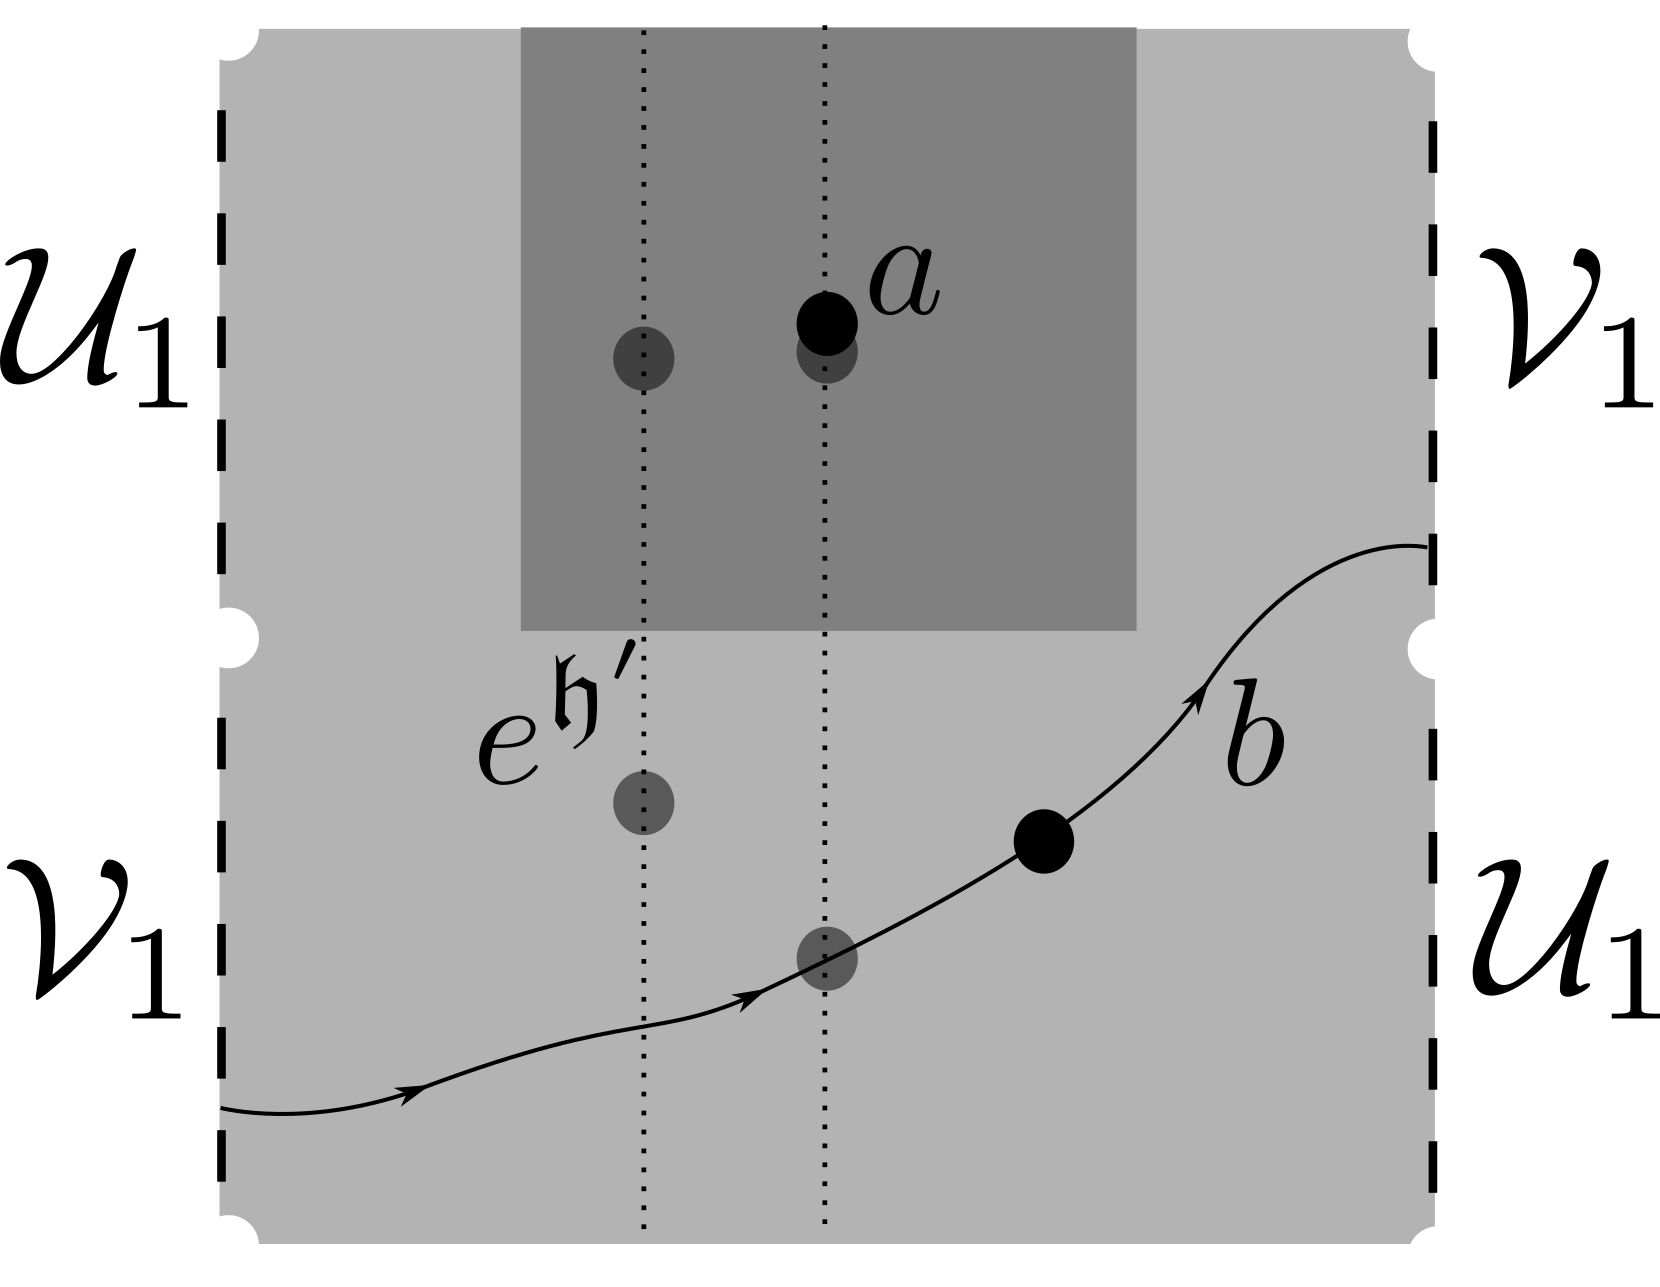
\includegraphics[scale=0.6]{counterexample.pdf}
 \caption{$\mu_*(a\otimes b)$ and $e^{\tup'}$ intersect once, transversely inside $C_2(\S)$.}
\label{fig:counterexample}
\end{figure}

Then the cycle $\kappa(p',\ualpha',\uu',\uv')$ consists uniquely of one tuple
\[
\tup'=(1,\ux'=(x'_1=2),\uu'=(u'_1=0),\uv'=(v'_1=0)).
\]
The corresponding cell $e^{\tup'}$ intersects once, transversely,
the cycle $\mu_*(a\otimes b)$, which is represented by the curve of configurations of two
points in $\mrS$, one of which is fixed at $a$ whereas the other runs along $b$:
there is exactly one position on $b$ lying under $a$.

Hence the algebraic intersection between these two classes is $1$, and since $p'>p$
this is an entry strictly above the diagonal in the matrix considered in the proof
of Lemma \ref{lem:oplussplitting}.

The proof of Theorem \ref{thm:Hbms*as*ggrep} can be easily generalised to surfaces
with more than one boundary curve. Let $\Sigma_{g,n}$ be a surface of genus
$g$ with $n\geq 1$ parametrised boundary curves and let $\Gamma_{g,n}$ be
the group of connected components of the topological group
$\Diff(\Sigma_{g,n};\partial\Sigma_{g,n})$:
then there is an isomorphism of bigraded $\Z_2$-representations
\begin{equation}
\label{eq:sgn}
\bigoplus_{m\geq 0}H_*\pa{C_m(\Sigma_{g,n})}\simeq \Z_2\left[Q^j\epsilon\,|\, j\geq 0\right]\otimes\Sym_{\bullet}(H_1(\Sigma_{g,n})),
\end{equation}

where the action of $\Gamma_{g,n}$ on the right-hand side is induced by the natural
action on $H_1(\Sigma_{g,n})$.

For $n\geq 2$ the intersection form on the vector space $H_1(\Sigma_{g,n})$
is \emph{degenerate}, but it is still invariant under the action of
$\Gamma_{g,n}$, so there is still a map from $\Gamma_{g,n}$ to the subgroup
of $GL_{2g+n-1}(\Z_2)$ fixing this bilinear form, and in this sense we can say
that the representation in \eqref{eq:sgn} is \emph{symplectic}.

The proof of the isomorphism \eqref{eq:sgn} is almost verbatim the same; the main difference is in the construction of the
model $\T(\Sigma_{g,n})$ for $\mathring{\Sigma}_{g,n}$: we divide the
vertical segments $\set{0,1}\times[0,1]\subset[0,1]^2$
into $2g+n-1$ equal parts, that we call $I_i^l$ and $I_i^r$ according to their order;
we identify, for each $i>2g$, the interval $I_i^l$ with the interval $I_i^r$;
the other couples of intervals, yielding the genus, are identified just as before.

One can further generalise to non-orientable surfaces with non-empty boundary: it suffices,
in the above construction, to glue some of the intervals $I_i^l$ and $I_i^r$ reversing their
orientation. We leave all details of these generalisations to the interested reader.